\documentclass[journal]{IEEEtran}

\usepackage[style=ieee]{biblatex} 
\usepackage{amsmath}
\usepackage{url}
\usepackage{graphicx}
\usepackage{float}

% \bibliography{example_bib.bib}

\begin{document}

\title{Investigating Cross-Sectional Size Distribution of Randomly Distributed 3D Spheres}

\author{Sai Pandian, ID:\@ 29899923}%
        
% The report headers
\markboth{PHYS6017 Computer Techniques in Physics Report 2, May 2020}
% do not delete next lines
{Shell \MakeLowercase{\textit{et al.}}: Bare Demo of IEEEtran.cls for IEEE Journals}

\maketitle

\begin{abstract}
  Text
\end{abstract}

\section{Introduction}

\IEEEPARstart{T}{ext}

\section{Materials and Methods}
Text


\section{Results}
Text

\begin{figure}[H]%[!ht]
\begin{center}
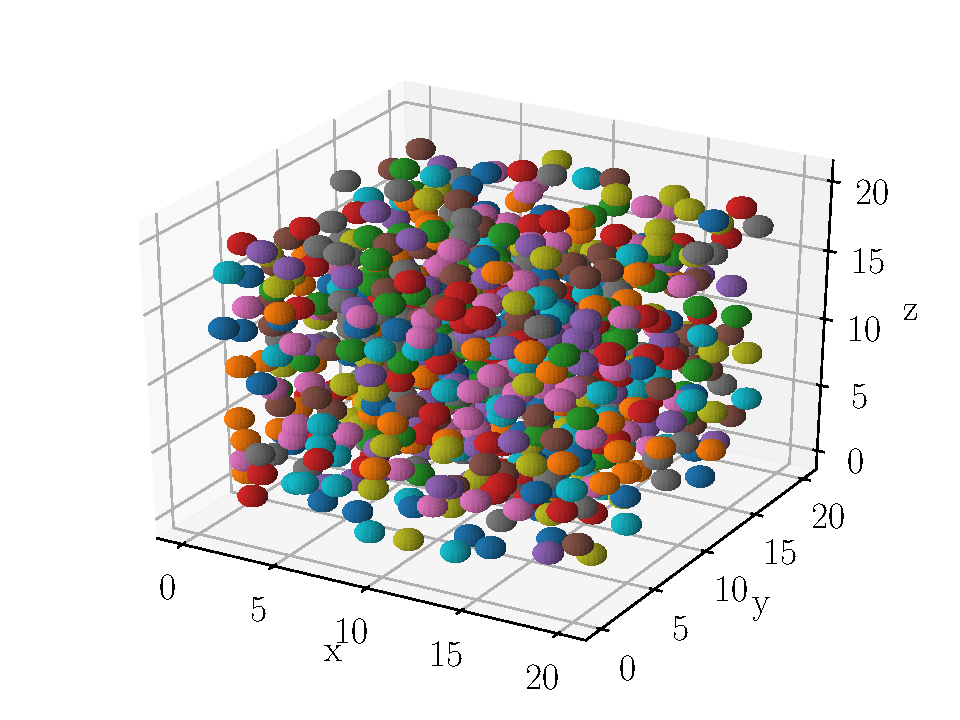
\includegraphics[width=0.45\textwidth]{./../Figures/box3d_noplane.pdf}
\caption{Illustrations, graphs, and photographs may fit across both columns, if
  necessary. Your artwork must be in place in the article.}
\label{fig:3dplot}
\end{center}
\end{figure}

\begin{figure}[H]%[!ht]
\begin{center}
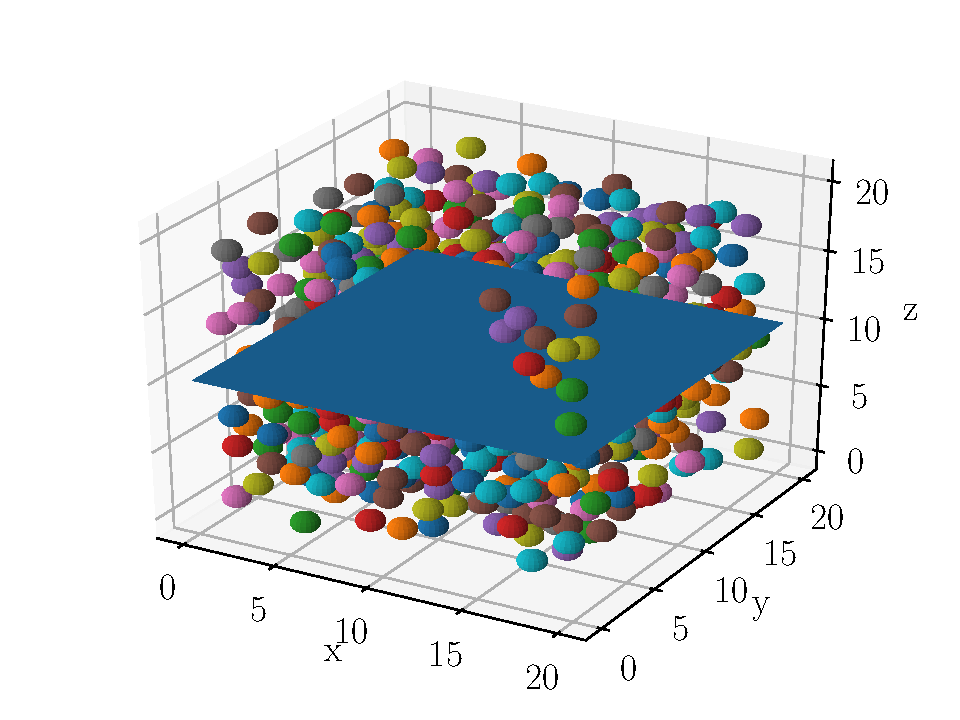
\includegraphics[width=0.45\textwidth]{./../Figures/box3d.pdf}
\caption{Illustrations, graphs, and photographs may fit across both columns, if
  necessary. Your artwork must be in place in the article.}
\label{fig:3dplot_plane}
\end{center}
\end{figure}

\begin{figure}[H]%[!ht]
\begin{center}
\includegraphics[width=0.45\textwidth]{./../Figures/circles.pdf}
\caption{Illustrations, graphs, and photographs may fit across both columns, if
  necessary. Your artwork must be in place in the article.}
\label{fig:circles}
\end{center}
\end{figure}

\begin{figure}[H]%[!ht]
\begin{center}
\includegraphics[width=0.45\textwidth]{./../Figures/750_01.pdf}
\caption{Illustrations, graphs, and photographs may fit across both columns, if
  necessary. Your artwork must be in place in the article.}
\label{fig:size1}
\end{center}
\end{figure}

\begin{figure}[H]%[!ht]
\begin{center}
\includegraphics[width=0.45\textwidth]{./../Figures/750_03.pdf}
\caption{Illustrations, graphs, and photographs may fit across both columns, if
  necessary. Your artwork must be in place in the article.}
\label{fig:size3}
\end{center}
\end{figure}

\begin{figure}[H]%[!ht]
\begin{center}
\includegraphics[width=0.45\textwidth]{./../Figures/750_07.pdf}
\caption{Illustrations, graphs, and photographs may fit across both columns, if
  necessary. Your artwork must be in place in the article.}
\label{fig:size7}
\end{center}
\end{figure}

\begin{figure}[H]%[!ht]
\begin{center}
\includegraphics[width=0.45\textwidth]{./../Figures/750_07_random.pdf}
\caption{Illustrations, graphs, and photographs may fit across both columns, if
  necessary. Your artwork must be in place in the article.}
\label{fig:random}
\end{center}
\end{figure}

\begin{figure}[H]%[!ht]
\begin{center}
\includegraphics[width=0.45\textwidth]{./../Figures/750_07_NoNoise.pdf}
\caption{Illustrations, graphs, and photographs may fit across both columns, if
  necessary. Your artwork must be in place in the article.}
\label{fig:nonoise}
\end{center}
\end{figure}

\begin{figure}[H]%[!ht]
\begin{center}
\includegraphics[width=0.45\textwidth]{./../Figures/750_07_Noise_100.pdf}
\caption{Illustrations, graphs, and photographs may fit across both columns, if
  necessary. Your artwork must be in place in the article.}
\label{fig:2noise}
\end{center}
\end{figure}

\begin{figure}[H]%[!ht]
\begin{center}
\includegraphics[width=0.45\textwidth]{./../Figures/750_07_Noise_10.pdf}
\caption{Illustrations, graphs, and photographs may fit across both columns, if
  necessary. Your artwork must be in place in the article.}
\label{fig:1noise}
\end{center}
\end{figure}

\section{Discussion and Summary}
Text



% if have a single appendix:
%\appendix[Proof of the Zonklar Equations]
% or
%\appendix  % for no appendix heading
% do not use \section anymore after \appendix, only \section*
% is possibly needed

% use appendices with more than one appendix
% then use \section to start each appendix
% you must declare a \section before using any
% \subsection or using \label (\appendices by itself
% starts a section numbered zero.)
%
\appendices{}
\section{Appendix Name}
Text

\printbibliography{}
\end{document}
